\documentclass[runningheads,10pt]{llncs}
%
\usepackage[T1]{fontenc}
%\documentclass[11pt]{article}

%\usepackage[margin=1in]{geometry}
\usepackage{amsmath,amssymb}
\usepackage{booktabs}
\usepackage{multirow}
\usepackage{array}
\usepackage{graphicx}
\usepackage{xcolor}
\usepackage{caption}
\usepackage{tikz}
\usepackage{pgfplots}
\pgfplotsset{compat=1.17}
\usepackage{quantikz}
\usepackage{hyperref}
\usepackage{enumitem}

\hypersetup{colorlinks=true, linkcolor=blue, citecolor=blue, urlcolor=blue}

%\newtheorem{definition}{Definition}
%\newtheorem{lemma}{Lemma}
%\newtheorem{proposition}{Proposition}
%\newtheorem{remark}{Remark}

\title{Quantum Resource Estimation for QARMA-64\\
\large Minimum-Toffoli S-boxes, Gidney AND Gadgets, and a Verified Grover Key-Search Oracle}
\author{}
\institute{}
\date{}

\begin{document}
\maketitle

\begin{abstract}
QARMA-64 is the tweakable block cipher behind pointer authentication in Armv8.3-A~\cite{avanzi2017qarma,qualcomm2017pac}, which makes the cost of attacking it on a quantum computer a practical question rather than an academic one. This paper gives a gate-level circuit for the cipher and a resource estimate in which every figure comes from a circuit that was actually built, simulated and checked. The S-box implementations we began with were produced by LIGHTER-R under a 9\,GB memory budget, and for the three odd S-boxes they contain a $C^3X$ gate whose textbook compilation costs 21 T gates on its own. Wanting that gate cheaper is what led us to Gidney's temporary-AND construction~\cite{gidney2018halving}, and much of what follows grew out of it. We first settle the Toffoli cost of the S-boxes. A meet-in-the-middle search over left cosets of the affine group shows exhaustively that $\sigma_1$ needs exactly 5 Toffoli gates without ancillas, while $\sigma_0$ and $\sigma_2$, being odd permutations, need one $C^3X$ alongside four Toffoli gates. The AND gadget is then applied, but only where a pair of Toffoli gates is provably clean: eligibility is decided by simulating all inputs, not by reading the circuit. On a RevKit-synthesised baseline that leaves 4 eligible pairs in $\sigma_1$ and takes its T-count from 175 to 135 (22.9\%). The in-place Toffoli gates left over are no obstacle either. One borrowed clean ancilla per cell implements any Toffoli with four T gates~\cite{jones2013lowoverhead,gidney2018halving}, an identity we verify exactly in both measurement branches. A single encryption ($\sigma_1$, $r=7$) then costs 8\,960 T gates on 192 qubits without ancillas, or 5\,120 T gates at T-depth 160 on 208 qubits with gadgets throughout: 42.9\% fewer T gates, 50.0\% less T-depth, and 8.8$\times$ fewer T gates than the baseline. One Grover iteration over three plaintext--ciphertext pairs uses 560 qubits at T-depth 334, which puts the whole key search at $2^{81.19}$ Clifford+T gates and depth $2^{75.19}$. The circuits are released as OpenQASM together with the scripts that regenerate every table.

\medskip
\noindent\textbf{Keywords:} QARMA, quantum cryptanalysis, Grover's algorithm, temporary AND, T-count, reversible circuit synthesis, resource estimation.
\end{abstract}

\section{Introduction}

Pointer authentication in Armv8.3-A computes its authentication codes with QARMA-64~\cite{avanzi2017qarma,qualcomm2017pac}, so the cipher ships on a very large number of devices. The generic quantum threat against it is Grover key search~\cite{grover1996fast}. That the attack exists is not in question; what matters is what running it would cost. Since Grassl et al.~\cite{grassl2016applying} and Jaques et al.~\cite{jaques2020implementing}, the accepted way to answer that is to build the oracle and count qubits, T gates and depth, which is also the language NIST uses for its security categories~\cite{nist2016submission}.

Two quantities govern the answer. One is the Toffoli count of the S-box, since the S-box layers carry all of the cipher's non-linearity. The other is how each Toffoli is compiled: seven T gates for the textbook decomposition, against four for Jones' measurement-based construction, and none at all for the matching uncomputation in Gidney's temporary-AND~\cite{jones2013lowoverhead,gidney2018halving}.

\paragraph{Contributions.} Three strands run through the paper.

\begin{enumerate}
\item \textbf{Exact Toffoli counts for the QARMA-64 S-boxes} (Section~\ref{sec:minimum-toffoli}). Ancilla-free NCT synthesis reduces to a search over left cosets of $\mathrm{AGL}(4,2)$ generated by what we call generalised Toffoli gates, of which there turn out to be exactly 420. Enumerating 291\,480 cosets at depth three makes a meet-in-the-middle search exhaustive, and it puts the Toffoli count of $\sigma_1$ at exactly 5, with $\sigma_0$ and $\sigma_2$ needing one $C^3X$ and four Toffoli gates. Unit tests on the coset canonicalisation and known-answer tests that recover planted circuits of known length guard against the search silently being wrong.

\item \textbf{AND gadgets used only where they are provably valid} (Section~\ref{sec:and-gadget-applied}). Clean compute/uncompute pairs are identified by simulating every input rather than by inspecting the circuit, and each rewritten circuit is re-checked in every measurement branch against the ideal permutation. In-place Toffoli gates, which have no clean target to write into, still admit the four-T construction if one clean ancilla per cell is borrowed.

\item \textbf{A cipher circuit and Grover oracle that were actually verified} (Sections~\ref{sec:full-circuit} and~\ref{sec:grover}). The encryption circuit reproduces all nine published test vectors across 39 configurations. The oracle marks the correct key and no wrong one, and hands back every work register untouched; the AND-tree comparator and the diffusion operator are exercised end to end by a small Grover run that reaches success probability 0.9966 and does not care what the random measurement outcomes were.
\end{enumerate}

Section~\ref{sec:sbox-implementations} reproduces the four LIGHTER-R implementations the project actually uses, with circuit diagrams and gate sequences, so that a reader can check them by hand instead of taking them on trust.

\paragraph{What is proven, and what is only the best we found.} The distinction is kept explicit throughout, because the two are easy to conflate. Proven are the Toffoli counts, within the circuit class stated (four wires, no ancillas, one $C^3X$ for the odd S-boxes), and the correctness of every gadget and circuit we use, established by simulation. Minimising Toffoli count and minimising T-count part  as soon as ancillas are permitted, and Section~\ref{sec:and-gadget-applied} shows by how much. We don't claim that the Tcount has global optimality.



\section{Preliminaries}

\subsection{Gates, cost metrics and the fault-tolerant model}

Reversible classical logic needs only the NCT library: $X$, $CX$ and the Toffoli gate $CCX$. Fault-tolerant hardware, on the other hand, implements Clifford+T, where the T gates dominate the bill because each one has to be distilled. Throughout we report width in qubits, gate counts at the NCT level, T-count, Clifford count, T-depth and full depth. Depths are obtained by scheduling the explicit gate list as early as possible, so two gates occupy the same layer only when they act on disjoint qubits. For attacks we add the G-cost (total gates) and the DW-cost (depth $\times$ width) of Jaques et al.~\cite{jaques2020implementing}.

\subsection{Grover key search}

Grover's algorithm~\cite{grover1996fast,boyer1998tight} recovers a $k$-bit key in $\left\lfloor \frac{\pi}{4} 2^{k/2} \right\rfloor$ iterations of $D O_f$ which is one complete iteration of Grover's algorithm. For a block cipher the oracle encrypts $s$ known plaintexts under the superposed key, compares the results against the known ciphertexts, and then undoes the encryptions. Parallelisation helps far less than one might think ~\cite{zalka1999grovers}: spreading the search over $S$ machines reduces the iteration count only by $\sqrt{S}$. That is why NIST caps circuit depth at $MAXDEPTH$ and quotes the AES-128 reference cost as $2^{170}/MAXDEPTH$  quantum gates~\cite{nist2016submission}.

\section{QARMA-64}

QARMA-64~\cite{avanzi2017qarma} takes a 64-bit plaintext, a 64-bit tweak and a 128-bit key $K = w^0 \| k^0$, and returns a 64-bit ciphertext. The construction is a three-round Even--Mansour scheme: $r$ forward rounds, then a keyed pseudo-reflector, then $r$ backward rounds that invert the forward ones (Figure~\ref{fig:qarma-encryption}). Its state is a $4\times4$ array of 4-bit cells. A forward round is
\[
R(IS, tk) = S \circ M \circ \tau(IS \oplus tk),
\]
except for the first, which omits $\tau$ and $M$. Here $\tau$ is the MIDORI cell permutation~\cite{banik2015midori} and $M = Q = \mathrm{circ}(0,\rho,\rho^2,\rho)$, with $\rho$ rotating a cell by one bit; note that $M^2 = I$. The tweak is updated by a cell permutation $h$ followed by a 4-bit LFSR $\omega$ applied to seven of the cells, and the whitening key satisfies $w^1 = o(w^0) = (w^0 \gg 1) \oplus (w^0 \gg 63)$, with $k^1 = k^0$ for encryption. Three S-boxes $\sigma_0, \sigma_1, \sigma_2$ are specified. We handle all three throughout and take $\sigma_1$ with $r=7$ as the primary instance. Our reference implementation was written from the specification alone; it reproduces all nine published test vectors (Table~\ref{tab:test-vectors}), which is what licenses us to use those vectors as a check on the circuits later.

\begin{figure}[htbp]
\centering
\resizebox{\textwidth}{!}{%
\begin{tikzpicture}[node distance=1.3cm, font=\normalsize, ->, >=Stealth]
 % ---- Row 1: forward half, up to the pseudo-reflector ----
 \node (P) {$P$};
 \node[right=of P] (w0) {$w^0$};
 \node[right=of w0] (R0) {$R_0^{\text{short}}$};
 \node[right=of R0] (dots1) {$\cdots$};
 \node[right=of dots1] (Rr1) {$R_{r-1}$};
 \node[right=of Rr1] (R) {$R$};
 \node[right=of R] (tau) {$\tau$};
 \node[right=of tau] (Q) {$Q$};
 \node[right=of Q] (k1) {$\oplus k^1$};

 % ---- Row 2: backward half, from the reflector to the ciphertext ----
 \node[below=1.6cm of P] (taui) {$\tau^{-1}$};
 \node[right=of taui] (R1) {$R$};
 \node[right=of R1] (dots2) {$\cdots$};
 \node[right=of dots2] (Rr1b) {$R_{r-1}$};
 \node[right=of Rr1b] (R0b) {$R_0^{\text{short}}$};
 \node[right=of R0b] (w1) {$w^1$};
 \node[right=of w1] (C) {$C$};

 % ---- arrows within each row ----
 \draw[->] (P)--(w0)--(R0)--(dots1)--(Rr1)--(R)--(tau)--(Q)--(k1);
 \draw[->] (taui)--(R1)--(dots2)--(Rr1b)--(R0b)--(w1)--(C);

 % ---- connector: wraps row 1's end down into row 2's start ----
 \draw[->] (k1.south) -- ++(0,-0.5) -| (taui.north);

 % ---- tweakey labels ----
 \node[below=2mm of R0, font=\scriptsize] {$tk_0$};
 \node[below=2mm of dots1, font=\scriptsize] {$tk_1 \ldots tk_{r-1}$};
 \node[below=2mm of R1, font=\scriptsize] {$\bar{tk}_{r-1} \ldots \bar{tk}_1$};
 \node[below=2mm of R0b, font=\scriptsize] {$\bar{tk}_0$};
\end{tikzpicture}%
}
\caption{QARMA-64 encryption. Round tweakeys are $tk_i = k^0 \oplus c_i \oplus T_i$ and
$\bar{tk}_i = tk_i \oplus \alpha$, where $T_i$ is the $i$-th tweak state.}
\label{fig:qarma-encryption}
\end{figure}

\begin{table}[htbp]
\centering
\caption{The QARMA-64 S-boxes, used throughout this paper (hexadecimal).}
\label{tab:sboxes}
\begin{tabular}{l*{16}{c}}
\toprule
$x$ & 0 & 1 & 2 & 3 & 4 & 5 & 6 & 7 & 8 & 9 & A & B & C & D & E & F \\
\midrule
$\sigma_0(x)$ & 0 & E & 2 & A & 9 & F & 8 & B & 6 & 4 & 3 & 7 & D & C & 1 & 5 \\
$\sigma_1(x)$ & A & D & E & 6 & F & 7 & 3 & 5 & 9 & 8 & 0 & C & B & 1 & 2 & 4 \\
$\sigma_2(x)$ & B & 6 & 8 & F & C & 0 & 9 & E & 3 & 7 & 4 & 5 & D & 2 & 1 & A \\
$\sigma_2^{-1}(x)$ & 5 & E & D & 8 & A & B & 1 & 9 & 2 & 6 & F & 0 & 4 & C & 7 & 3 \\
\bottomrule
\end{tabular}
\end{table}

\section{The S-box Implementations We Started From}
\label{sec:sbox-implementations}

Our starting point was not a hand-built circuit. The four S-box implementations used in this project were generated with LIGHTER-R~\cite{dasu2019lighterr}, a synthesis tool for reversible $4\times4$ S-box circuits, running under its \texttt{MCT\_qc} gate library. The Two important features are as follows.

The first is,  The search was limited by the memory of the machine it ran on, which had 9\,GB of RAM; LIGHTER-R's exploration consumes a lot of memory, and once the memory  is gone the search stops . The circuits below are therefore the best found under that constraint, not globally optimal ones, and we claim nothing more for them -- neither in LIGHTER-R's own cost metric nor in ours. The Toffoli counts of all four circuits are as follows: five for $\sigma_1$, and four together with a single $C^3X$ for $\sigma_0$, $\sigma_2$ and $\sigma_2^{-1}$. On the one metric that governs T-cost, then, the memory limit cost us nothing at all. Their Clifford counts are in fact lower than those of our own synthesis, 8 CNOT and 2 NOT for $\sigma_1$ against our 18 and 5, which is a useful corrective to keep in mind when reading Table~\ref{tab:sbox-circuits}.

The second feature is the one that shaped this paper. Since \texttt{MCT\_qc} contains multi-controlled Toffoli gates, LIGHTER-R returns a $C^3X$ gate -- printed as \texttt{CCCNOT2} -- in three of the four circuits. It could hardly do otherwise, because $\sigma_0$, $\sigma_2$ and $\sigma_2^{-1}$ are odd permutations, and Lemma~\ref{lem:even-permutation} rules out any implementation built from NOT, CNOT and Toffoli gates alone on four wires. The problem is that a $C^3X$ is not a gate fault-tolerant hardware performs directly. Compiled the usual way it becomes three Toffoli gates acting on one clean ancilla, or 21 T gates, which is more than everything else in the S-box put together. Removing that overhead is where this line of work started.

 The ancilla of a $C^3X$ is written once, read as a control, and cleared again: it begins in $|0\rangle$, takes the value $a \wedge b$, and returns to $|0\rangle$. Gidney's temporary-AND construction was designed for compute/uncompute pairs of exactly this shape~\cite{gidney2018halving}, so it applies with nothing to adapt, and the $C^3X$ falls from 21 T gates to $4+7+0=11$. Once that substitution is made, the obvious question is whether the ordinary Toffoli gates admit the same treatment. Section~\ref{sec:in-place-toffoli} shows that they do, at the cost of one borrowed ancilla each, and the rest of the paper follows from there.


\paragraph{What we verified.} Each file was checked three separate ways, and all four pass every check. The \texttt{from} words decode to the identity permutation. The \texttt{to} words decode to the S-box truth table of Table~\ref{tab:sboxes}. And simulating the printed gate sequence, relabellings included, reproduces the S-box on all 16 inputs. The T-counts in Table~\ref{tab:lighterr-summary} correspond to the three compilation modes used later in Section~\ref{sec:and-gadget-applied}: every Toffoli and $C^3X$ compiled the textbook way; the $C^3X$ ancilla treated as the clean AND pair it is; and finally every Toffoli given a borrowed ancilla as well. Since these circuits carry the same Toffoli and $C^3X$ counts as the minimal ones of Section~\ref{sec:minimum-toffoli}, substituting them changes no T-count, T-depth or Grover figure anywhere in this paper. Only the Clifford counts move, and they move downwards.

\begin{table}[htbp]
\centering
\caption{The four LIGHTER-R implementations used in the project. ``Cost'' is LIGHTER-R's own metric as printed in each file. T-counts are for one S-box under the three compilation modes of Section~\ref{sec:and-gadget-applied}.}
\label{tab:lighterr-summary}
\small
\begin{tabular}{llccccccccc}
\toprule
S-box & File & Cost & NOT & CNOT & CCNOT & $C^3X$ & $T_{\text{textbook}}$ & $T_{\text{AND on }C^3X}$ & $T_{\text{AND everywhere}}$ \\
\midrule
$\sigma_0$ & \texttt{sigma0\_3} & 38 & 0 & 5 & 4 & 1 & 49 & 39 & 24 \\
$\sigma_1$ & \texttt{sigma1\_0} & 35 & 2 & 8 & 5 & 0 & 35 & 35 & 20 \\
$\sigma_2$ & \texttt{sigma2\_1} & 42 & 2 & 7 & 4 & 1 & 49 & 39 & 24 \\
$\sigma_2^{-1}$ & \texttt{sigma3\_0} & 42 & 1 & 8 & 4 & 1 & 49 & 39 & 24 \\
\bottomrule
\end{tabular}
\end{table}

\begin{figure}[htbp]
\centering
\begin{quantikz}
\lstick{$F_0=X_1$} & \targ{} & \qw \rstick{$X_0$} \\
\lstick{$F_1=X_0$} & \ctrl{-1} & \qw \rstick{$X_3$} \\
\lstick{$F_2=X_3$} & \qw & \qw \rstick{$X_1$} \\
\lstick{$F_3=X_2$} & \qw & \qw \rstick{$X_2$}
\end{quantikz}
\caption{Schematic wiring for $\sigma_0$ (file \texttt{implementation\_sigma0\_3.c}). Input labels give the initial relabelling $F[i]=X[j]$, output labels the final one $X[k]=F[i]$; $X_0$ is the most significant bit. Encoded input \texttt{00FF 0F0F 3333 5555} (the identity), output \texttt{5F0C 44DD 75B0 0D3B}. The full ten-gate sequence is given in Table~\ref{tab:sigma0-gates}.}
\label{fig:sigma0-circuit}
\end{figure}

\begin{table}[htbp]
\centering
\caption{Gate sequence for $\sigma_0$, exactly as printed by LIGHTER-R, with the corresponding gate in the notation of this paper. Applied top to bottom.}
\label{tab:sigma0-gates}
\small
\begin{tabular}{cll}
\toprule
\# & LIGHTER-R output line & Gate \\
\midrule
1 & \texttt{F[1] = CCNOT2(F[3], F[2], F[1]);} & $CCX(F_3,F_2 \to F_1)$ \\
2 & \texttt{F[3] = CNOT1(F[3], F[1]);} & $CX(F_1 \to F_3)$ \\
3 & \texttt{F[3] = CNOT1(F[3], F[2]);} & $CX(F_2 \to F_3)$ \\
4 & \texttt{F[2] = CCNOT2(F[3], F[1], F[2]);} & $CCX(F_3,F_1 \to F_2)$ \\
5 & \texttt{F[3] = CCCNOT2(F[0], F[1], F[2], F[3]);} & $C^3X(F_0,F_1,F_2 \to F_3)$ \\
6 & \texttt{F[3] = CNOT1(F[3], F[0]);} & $CX(F_0 \to F_3)$ \\
7 & \texttt{F[1] = CNOT1(F[1], F[2]);} & $CX(F_2 \to F_1)$ \\
8 & \texttt{F[0] = CCNOT2(F[3], F[1], F[0]);} & $CCX(F_3,F_1 \to F_0)$ \\
9 & \texttt{F[1] = CCNOT2(F[3], F[0], F[1]);} & $CCX(F_3,F_0 \to F_1)$ \\
10 & \texttt{F[3] = CNOT1(F[3], F[1]);} & $CX(F_1 \to F_3)$ \\
\bottomrule
\end{tabular}
\end{table}

\begin{figure}[htbp]
\centering
\begin{quantikz}
\lstick{$F_0=X_0$} & \qw & \qw \rstick{$X_2$} \\
\lstick{$F_1=X_1$} & \qw & \qw \rstick{$X_0$} \\
\lstick{$F_2=X_2$} & \qw & \qw \rstick{$X_1$} \\
\lstick{$F_3=X_3$} & \qw & \qw \rstick{$X_3$}
\end{quantikz}
\caption{Schematic wiring for $\sigma_1$ (file \texttt{implementation\_sigma1\_0.c}). Input labels give the initial relabelling $F[i]=X[j]$, output labels the final one $X[k]=F[i]$; $X_0$ is the most significant bit. Encoded input \texttt{00FF 0F0F 3333 5555} (the identity), output \texttt{E8D8 7D11 BE0A 4F8C}. The full fifteen-gate sequence is given in Table~\ref{tab:sigma1-gates}.}
\label{fig:sigma1-circuit}
\end{figure}

\begin{table}[htbp]
\centering
\caption{Gate sequence for $\sigma_1$, exactly as printed by LIGHTER-R, with the corresponding gate in the notation of this paper. Applied top to bottom.}
\label{tab:sigma1-gates}
\small
\begin{tabular}{cll}
\toprule
\# & LIGHTER-R output line & Gate \\
\midrule
1 & \texttt{F[3] = CNOT1(F[3], F[1]);} & $CX(F_1 \to F_3)$ \\
2 & \texttt{F[3] = CNOT1(F[3], F[0]);} & $CX(F_0 \to F_3)$ \\
3 & \texttt{F[0] = CCNOT2(F[3], F[2], F[0]);} & $CCX(F_3,F_2 \to F_0)$ \\
4 & \texttt{F[2] = CNOT1(F[2], F[1]);} & $CX(F_1 \to F_2)$ \\
5 & \texttt{F[3] = CCNOT2(F[1], F[0], F[3]);} & $CCX(F_1,F_0 \to F_3)$ \\
6 & \texttt{F[1] = CCNOT2(F[3], F[2], F[1]);} & $CCX(F_3,F_2 \to F_1)$ \\
7 & \texttt{F[2] = CCNOT2(F[1], F[0], F[2]);} & $CCX(F_1,F_0 \to F_2)$ \\
8 & \texttt{F[0] = RNOT1(F[0]);} & $X(F_0)$ \\
9 & \texttt{F[0] = CNOT1(F[0], F[1]);} & $CX(F_1 \to F_0)$ \\
10 & \texttt{F[2] = CNOT1(F[2], F[0]);} & $CX(F_0 \to F_2)$ \\
11 & \texttt{F[3] = CNOT1(F[3], F[1]);} & $CX(F_1 \to F_3)$ \\
12 & \texttt{F[0] = CCNOT2(F[3], F[2], F[0]);} & $CCX(F_3,F_2 \to F_0)$ \\
13 & \texttt{F[2] = CNOT1(F[2], F[1]);} & $CX(F_1 \to F_2)$ \\
14 & \texttt{F[1] = RNOT1(F[1]);} & $X(F_1)$ \\
15 & \texttt{F[2] = CNOT1(F[2], F[0]);} & $CX(F_0 \to F_2)$ \\
\bottomrule
\end{tabular}
\end{table}

\begin{figure}[htbp]
\centering
\begin{quantikz}
\lstick{$F_0=X_1$} & \qw & \qw \rstick{$X_3$} \\
\lstick{$F_1=X_2$} & \qw & \qw \rstick{$X_2$} \\
\lstick{$F_2=X_0$} & \qw & \qw \rstick{$X_0$} \\
\lstick{$F_3=X_3$} & \qw & \qw \rstick{$X_1$}
\end{quantikz}
\caption{Schematic wiring for $\sigma_2$ (file \texttt{implementation\_sigma2\_1.c}). Input labels give the initial relabelling $F[i]=X[j]$, output labels the final one $X[k]=F[i]$; $X_0$ is the most significant bit. Encoded input \texttt{00FF 0F0F 3333 5555} (the identity), output \texttt{BB09 5978 D1C5 92DA}. The full fourteen-gate sequence is given in Table~\ref{tab:sigma2-gates}.}
\label{fig:sigma2-circuit}
\end{figure}

\begin{table}[htbp]
\centering
\caption{Gate sequence for $\sigma_2$, exactly as printed by LIGHTER-R, with the corresponding gate in the notation of this paper. Applied top to bottom.}
\label{tab:sigma2-gates}
\small
\begin{tabular}{cll}
\toprule
\# & LIGHTER-R output line & Gate \\
\midrule
1 & \texttt{F[2] = CCNOT2(F[3], F[1], F[2]);} & $CCX(F_3,F_1 \to F_2)$ \\
2 & \texttt{F[0] = CNOT1(F[0], F[2]);} & $CX(F_2 \to F_0)$ \\
3 & \texttt{F[2] = CNOT1(F[2], F[1]);} & $CX(F_1 \to F_2)$ \\
4 & \texttt{F[3] = CNOT1(F[3], F[2]);} & $CX(F_2 \to F_3)$ \\
5 & \texttt{F[2] = CCNOT2(F[3], F[0], F[2]);} & $CCX(F_3,F_0 \to F_2)$ \\
6 & \texttt{F[3] = CCNOT2(F[2], F[1], F[3]);} & $CCX(F_2,F_1 \to F_3)$ \\
7 & \texttt{F[1] = CCCNOT2(F[0], F[2], F[3], F[1]);} & $C^3X(F_0,F_2,F_3 \to F_1)$ \\
8 & \texttt{F[1] = RNOT1(F[1]);} & $X(F_1)$ \\
9 & \texttt{F[2] = CNOT1(F[2], F[3]);} & $CX(F_3 \to F_2)$ \\
10 & \texttt{F[3] = CNOT1(F[3], F[0]);} & $CX(F_0 \to F_3)$ \\
11 & \texttt{F[0] = RNOT1(F[0]);} & $X(F_0)$ \\
12 & \texttt{F[0] = CNOT1(F[0], F[2]);} & $CX(F_2 \to F_0)$ \\
13 & \texttt{F[2] = CNOT1(F[2], F[1]);} & $CX(F_1 \to F_2)$ \\
14 & \texttt{F[1] = CCNOT2(F[3], F[2], F[1]);} & $CCX(F_3,F_2 \to F_1)$ \\
\bottomrule
\end{tabular}
\end{table}

\begin{figure}[htbp]
\centering
\begin{quantikz}
\lstick{$F_0=X_0$} & \qw & \qw \rstick{$X_3$} \\
\lstick{$F_1=X_1$} & \qw & \qw \rstick{$X_1$} \\
\lstick{$F_2=X_2$} & \qw & \qw \rstick{$X_2$} \\
\lstick{$F_3=X_3$} & \targ{} & \qw \rstick{$X_0$}
\end{quantikz}
\caption{Schematic wiring for $\sigma_2^{-1}$ (file \texttt{implementation\_sigma3\_0.c}). Input labels give the initial relabelling $F[i]=X[j]$, output labels the final one $X[k]=F[i]$; $X_0$ is the most significant bit. Encoded input \texttt{00FF 0F0F 3333 5555} (the identity), output \texttt{7D24 E06E 4CE3 A723}. The full fourteen-gate sequence is given in Table~\ref{tab:sigma3inv-gates}.}
\label{fig:sigma3inv-circuit}
\end{figure}

\begin{table}[htbp]
\centering
\caption{Gate sequence for $\sigma_2^{-1}$, exactly as printed by LIGHTER-R, with the corresponding gate in the notation of this paper. Applied top to bottom.}
\label{tab:sigma3inv-gates}
\small
\begin{tabular}{cll}
\toprule
\# & LIGHTER-R output line & Gate \\
\midrule
1 & \texttt{F[2] = CNOT1(F[2], F[3]);} & $CX(F_3 \to F_2)$ \\
2 & \texttt{F[3] = CNOT1(F[3], F[1]);} & $CX(F_1 \to F_3)$ \\
3 & \texttt{F[0] = CNOT1(F[0], F[3]);} & $CX(F_3 \to F_0)$ \\
4 & \texttt{F[2] = CCNOT2(F[1], F[0], F[2]);} & $CCX(F_1,F_0 \to F_2)$ \\
5 & \texttt{F[0] = CNOT1(F[0], F[2]);} & $CX(F_2 \to F_0)$ \\
6 & \texttt{F[1] = CNOT1(F[1], F[0]);} & $CX(F_0 \to F_1)$ \\
7 & \texttt{F[3] = RNOT1(F[3]);} & $X(F_3)$ \\
8 & \texttt{F[2] = CCCNOT2(F[0], F[1], F[3], F[2]);} & $C^3X(F_0,F_1,F_3 \to F_2)$ \\
9 & \texttt{F[1] = CCNOT2(F[3], F[2], F[1]);} & $CCX(F_3,F_2 \to F_1)$ \\
10 & \texttt{F[3] = CCNOT2(F[1], F[0], F[3]);} & $CCX(F_1,F_0 \to F_3)$ \\
11 & \texttt{F[0] = CNOT1(F[0], F[3]);} & $CX(F_3 \to F_0)$ \\
12 & \texttt{F[3] = CNOT1(F[3], F[2]);} & $CX(F_2 \to F_3)$ \\
13 & \texttt{F[1] = CNOT1(F[1], F[3]);} & $CX(F_3 \to F_1)$ \\
14 & \texttt{F[3] = CCNOT2(F[1], F[0], F[3]);} & $CCX(F_1,F_0 \to F_3)$ \\
\bottomrule
\end{tabular}
\end{table}

\section{The Temporary-AND Gadget}
\label{sec:temp-and}

Gidney's temporary-AND~\cite{gidney2018halving}, which builds on Jones' measurement-based Toffoli construction~\cite{jones2013lowoverhead}, computes the logical AND of two controls into a fresh ancilla using four T gates, then erases that ancilla later at no T cost whatsoever:

\begin{itemize}
\item \textbf{compute} (Figure~\ref{fig:toffoli-constructions}b): thirteen gates, namely 2$H$, 2$T$, 2$T^\dagger$, 6$CX$ and 1$S$, taking $|a,b,0\rangle$ to $|a,b,ab\rangle$. This is exact rather than relative-phase, as we checked: on all four inputs with the target in $|0\rangle$ the output amplitude is precisely $+1$.
\item \textbf{uncompute}: measure the ancilla in the $X$ basis, then apply a classically controlled $CZ$ to the two controls and reset the ancilla. No T gates are involved. Both outcomes occur with probability exactly $1/2$, and we confirmed that either one restores the input state exactly.
\end{itemize}

Rather than transcribe the circuit from the paper, we took the gate list from the reference implementation in Qualtran~\cite{harrigan2024expressing} (\texttt{qualtran.bloqs.mcmt.and\_bloq.And}) and re-verified it as an $8\times8$ unitary.

\begin{remark}[model assumption]
Measurement-based uncomputation needs mid-circuit measurement and classical feed-forward inside the coherence budget. Surface-code cost models take this for granted~\cite{gidney2018halving,jaques2020implementing}, but it is a genuine assumption : on hardware without adaptive control the zero-T uncomputation is not possible to implement, and the `textbook' columns of our tables are the ones to read.
\end{remark}

\begin{table}[htbp]
\centering
\caption{Cost of one Toffoli-equivalent, as measured on the circuits themselves.}
\label{tab:toffoli-cost}
\small
\begin{tabular}{lccccll}
\toprule
Construction & Ancilla & T-count & T-depth & Clifford & Meas. & Notes \\
\midrule
Toffoli (textbook, Nielsen--Chuang) & 0 & 7 & 4 & 8 & 0 & exact \\
AND compute (Gidney/Qualtran) & 1 clean & 4 & 2 & 9 & 0 & exact, target must be $|0\rangle$ \\
AND uncompute & -- & 0 & 0 & 2 & 1 & measurement based \\
Toffoli via AND + borrowed ancilla & 1 clean & 4 & 2 & 12 & 1 & exact, any target \\
\bottomrule
\end{tabular}
\end{table}

\begin{figure}[htbp]
\centering
\textbf{(a)} Textbook Toffoli: 7 T, T-depth 4.
\[
\begin{quantikz}
\lstick{$a$} & \ctrl{2} & \qw & \qw & \qw & \qw & \qw & \ctrl{2} & \qw & \qw & \qw \rstick{$a$}\\
\lstick{$b$} & \qw & \ctrl{1} & \qw & \qw & \qw & \ctrl{1} & \qw & \qw & \qw & \qw \rstick{$b$}\\
\lstick{$t$} & \targ{} & \targ{} & \gate{T^\dagger} & \targ{} & \gate{T} & \targ{} & \targ{} & \gate{T} & \gate{H} & \qw \rstick{$t\oplus ab$}
\end{quantikz}
\]

\medskip
\textbf{(b)} AND compute (Gidney/Qualtran): 4 T, T-depth 2.
\[
\begin{quantikz}
\lstick{$a$} & \ctrl{1} & \gate{T} & \ctrl{2} & \qw & \qw \rstick{$a$}\\
\lstick{$b$} & \targ{} & \gate{T} & \qw & \ctrl{1} & \qw \rstick{$b$}\\
\lstick{$|0\rangle$} & \qw & \gate{H} & \targ{} & \targ{} & \gate{S}\rstick{$|ab\rangle$}
\end{quantikz}
\]

\medskip
\textbf{(c)} Any in-place Toffoli with 4 T gates, by borrowing one clean ancilla. $\wedge$ is the AND compute of (b) and $\wedge^\dagger$ its measurement-based uncomputation.
\[
\begin{quantikz}
\lstick{$a$} & \qwbundle{} & \gate[3]{\wedge}\qwbundle{} & \qw & \gate[3]{\wedge^\dagger}\qwbundle{} & \qw \rstick{$a$}\\
\lstick{$b$} & & & \ctrl{1} & & \qw \rstick{$b$}\\
\lstick{$t$} & & & \targ{} & & \qw \rstick{$t \oplus ab$}
\end{quantikz}
\quad
\text{(ancilla starts and ends in $|0\rangle$)}
\]
\caption{Toffoli implementations used in this paper; all three were verified exactly (Section~\ref{sec:verification}).}
\label{fig:toffoli-constructions}
\end{figure}

\section{Minimum-Toffoli S-box Circuits}
\label{sec:minimum-toffoli}

\subsection{Reduction to generalised Toffoli gates}

Let $\mathrm{AGL}(4,2)$ be the affine group on $\mathbb{F}_2^4$, of order $322\,560$; its elements are exactly the permutations realisable with CNOT and NOT gates alone.

\begin{definition}
A \emph{generalised Toffoli gate} is a permutation $B\,CCX\,B^{-1}$ with $B \in \mathrm{AGL}(4,2)$.
\end{definition}

Any ancilla-free NCT circuit with $t$ Toffoli gates can be written $A_t CCX A_{t-1} \cdots CCX A_0$ with the $A_i$ affine. Inserting $B_i B_i^{-1}$ between the factors turns this into $A \circ G_1 \circ \cdots \circ G_t$ with each $G_i$ a generalised Toffoli gate, and the rewriting runs equally well in reverse. The Toffoli count of $\pi$ is therefore the smallest $t$ for which the left coset $\mathrm{AGL}(4,2)\circ\pi$ contains a product of $t$ generalised Toffoli gates. Enumerating them gives 420 such gates, each with a stabiliser of order 768.

Left cosets are canonicalised by translating so that $\pi(0)=0$ and then mapping the first four linearly independent images onto the unit vectors. Breadth-first search from the identity coset reaches $105$, $6\,510$ and $291\,480$ new cosets at depths 1, 2 and 3 respectively. A second search, started from the target, meets that table in the middle. Both halves are exhaustive, so the answer they produce is exhaustive too.

\begin{lemma}
\label{lem:even-permutation}
Every NCT gate on four wires induces an even permutation of $\mathbb{F}_2^4$; hence an odd permutation has no ancilla-free NCT implementation on four wires.
\end{lemma}
\begin{proof}
On four wires $X$ is a product of 8 transpositions, $CX$ of 4 and $CCX$ of 2.
\end{proof}

As it happens $\sigma_1$ is a fixed-point-free involution, hence a product of 8 transpositions and even, whereas $\sigma_0$ and $\sigma_2$ are odd. For the odd cases we therefore search for $\pi = A \circ G_1 \cdots G_t \circ \theta$, where $\theta$ is an affine conjugate of $C^3X$, which is to say an arbitrary transposition.

\begin{proposition}
\label{prop:min-toffoli}
The Toffoli count of $\sigma_1$ over ancilla-free NCT circuits is exactly 5. $\sigma_0$, $\sigma_2$ and $\sigma_2^{-1}$ have no such circuit; with exactly one $C^3X$ gate their minimum Toffoli count is 4.
\end{proposition}
\begin{proof}
Exhaustive search as above: no decomposition with at most 4 generalised Toffoli gates exists for $\sigma_1$, and 640 decompositions with 5 do; for $\sigma_0$ and $\sigma_2$ (composed with a transposition) none with at most 3 exists and 312 resp.\ 160 exist with 4. $\sigma_2^{-1}$ follows by reversing the circuit.
\end{proof}

\begin{remark}[scope]
Proposition~\ref{prop:min-toffoli} is a statement about four wires and no ancillas. Nothing here rules out a smaller Toffoli count once ancillas are allowed; that space was never searched. And as Section~\ref{sec:and-gadget-applied} makes clear, ancillas change the T-count picture considerably even when the Toffoli count stays put.
\end{remark}

\subsection{From decompositions to gate sequences}


\begin{figure}[htbp]
\centering
\textbf{(a)} Ancilla-free: 5 Toffoli, 18 CNOT, 5 NOT; T-count 35, T-depth 20.\\[4pt]
\textbf{(b)} Same circuit with every Toffoli replaced by an AND gadget on one borrowed ancilla: T-count 20, T-depth 10.
\caption{Circuits for $\sigma_1$ ($x_0$ is the least significant bit); the exact gate sequence is given in Table~\ref{tab:sigma1-full-gates}. Since $\sigma_1$ is an involution, each also implements $\sigma_1^{-1}$.}
\label{fig:sigma1-full}
\end{figure}

\section{Applying the AND Gadget}
\label{sec:and-gadget-applied}

\subsection{What must be proven}

An AND gadget may stand in for a pair of Toffoli gates only when that pair really is a clean compute/uncompute pair, and  A candidate pair $(i,j)$ on controls $a,b$ with target $t$ is accepted only if, for every input: (i) $t$ holds $|0\rangle$ immediately before gate $i$; (ii) the next gate that targets $t$ after $i$ is exactly gate $j$, with the same controls; (iii) $a$ and $b$ keep their values between $i$ and $j$; (iv) $t$ holds $a \wedge b$ at gate $j$ and returns to $|0\rangle$ afterwards. 

Run against a RevKit-synthesised baseline~\cite{soeken2012revkit}, the test accepts 4 pairs in $\sigma_1$. Every rejected candidate fails for the same reason, namely that its target is not $|0\rangle$ before the compute, so the rejects are precisely the in-place Toffoli gates (Table~\ref{tab:clean-and-pairs}). The T-count of $\sigma_1$ drops from 175 to 135, a saving of 22.9\%.

\begin{table}[htbp]
\centering
\caption{Verified clean AND pairs in the RevKit baseline circuits. Rejected candidates are in-place Toffoli gates (target not $|0\rangle$).}
\label{tab:clean-and-pairs}
\small
\begin{tabular}{lcccccc}
\toprule
S-box & Toffoli gates & verified pairs & rejected & $T$ (textbook) & $T$ (AND pairs) & reduction \\
\midrule
$\sigma_0$ & 30 & 5 & 20 & 210 & 160 & 23.8\% \\
$\sigma_1$ & 25 & 4 & 17 & 175 & 135 & 22.9\% \\
$\sigma_2$ & 28 & 5 & 18 & 196 & 146 & 25.5\% \\
$\sigma_2^{-1}$ & 19 & 3 & 13 & 133 & 103 & 22.6\% \\
\bottomrule
\end{tabular}
\end{table}

\subsection{In-place Toffoli gates are not an obstacle}
\label{sec:in-place-toffoli}

What the test rejects, then, are the in-place Toffoli gates, whose targets carry data that no AND gadget may overwrite. Even those need not pay for the 7-T decomposition. Borrow a single clean ancilla $g$ and write
\begin{equation}
CCX(a,b \to t) = \mathrm{AND}(a,b \to g)\,;\ CX(g\to t)\,;\ \mathrm{AND}^\dagger(a,b\to g),
\label{eq:borrowed-toffoli}
\end{equation}
at a cost of 4 T gates, T-depth 2, one measurement and one additional CNOT (Figure~\ref{fig:toffoli-constructions}c). This is nothing more than Jones' measurement-based Toffoli~\cite{jones2013lowoverhead} written out with Gidney's gadget~\cite{gidney2018halving}, and we claim no novelty for it; what is ours is the systematic application and the checking. 

A single borrowed ancilla per S-box is enough, since the Toffoli gates within a cell run one after another; the 16 cells of a layer then proceed in parallel on 16 ancillas. $\sigma_0$ and $\sigma_2$ want a second ancilla per cell, because the first is still tied up by the $C^3X$ when its inner Toffoli executes. Table~\ref{tab:sbox-circuits} and Figure~\ref{fig:tcount-per-sbox} collect the effect. For $\sigma_1$ the T-count falls from 35 to 20 and the T-depth from 20 to 10.

\begin{table}[htbp]
\centering
\caption{S-box circuits. `Textbook' compiles every Toffoli with 7 T gates; `AND pairs' uses gadgets only where provably valid; `AND everywhere' additionally applies Equation~\eqref{eq:borrowed-toffoli}. Depth is the full Clifford+T depth.}
\label{tab:sbox-circuits}
\scriptsize
\begin{tabular}{llccccccc}
\toprule
S-box & Implementation & Qubits & Toffoli & AND & CNOT & NOT & T-count & T-depth \\
& & & & & & & & (Depth) \\
\midrule
\multirow{6}{*}{$\sigma_0$}
& RevKit, textbook 7-T & 5 & 30 & 0 & 9 & 0 & 210 & 119 (323) \\
& RevKit, AND pairs & 5 & 20 & 5 & 9 & 0 & 160 & 90 (288) \\
& RevKit, AND everywhere & 6 & 0 & 25 & 29 & 0 & 100 & 45 (344) \\
& This work, textbook 7-T & 5 & 7 & 0 & 17 & 7 & 49 & 27 (87) \\
& This work, AND pairs & 5 & 5 & 1 & 17 & 7 & 39 & 21 (78) \\
& This work, AND everywhere & 6 & 0 & 6 & 22 & 7 & 24 & 11 (93) \\
\midrule
\multirow{6}{*}{$\sigma_1$}
& RevKit, textbook 7-T & 5 & 25 & 0 & 10 & 2 & 175 & 99 (268) \\
& RevKit, AND pairs & 5 & 17 & 4 & 10 & 2 & 135 & 76 (240) \\
& RevKit, AND everywhere & 6 & 0 & 21 & 27 & 2 & 84 & 38 (293) \\
& This work, textbook 7-T & 4 & 5 & 0 & 18 & 5 & 35 & 20 (71) \\
& This work, AND pairs & 4 & 5 & 0 & 18 & 5 & 35 & 20 (71) \\
& This work, AND everywhere & 5 & 0 & 5 & 23 & 5 & 20 & 10 (79) \\
\midrule
\multirow{6}{*}{$\sigma_2$}
& RevKit, textbook 7-T & 5 & 28 & 0 & 9 & 2 & 196 & 111 (300) \\
& RevKit, AND pairs & 5 & 18 & 5 & 9 & 2 & 146 & 82 (265) \\
& RevKit, AND everywhere & 6 & 0 & 23 & 27 & 2 & 92 & 41 (316) \\
& This work, textbook 7-T & 5 & 7 & 0 & 18 & 5 & 49 & 27 (89) \\
& This work, AND pairs & 5 & 5 & 1 & 18 & 5 & 39 & 21 (82) \\
& This work, AND everywhere & 6 & 0 & 6 & 23 & 5 & 24 & 11 (95) \\
\midrule
\multirow{3}{*}{$\sigma_2^{-1}$}
& RevKit, textbook 7-T & 5 & 19 & 0 & 14 & 2 & 133 & 76 (213) \\
& RevKit, AND pairs & 5 & 13 & 3 & 14 & 2 & 103 & 58 (192) \\
& RevKit, AND everywhere & 6 & 0 & 16 & 27 & 2 & 64 & 29 (225) \\
\bottomrule
\end{tabular}
\end{table}

\begin{figure}[htbp]
\centering
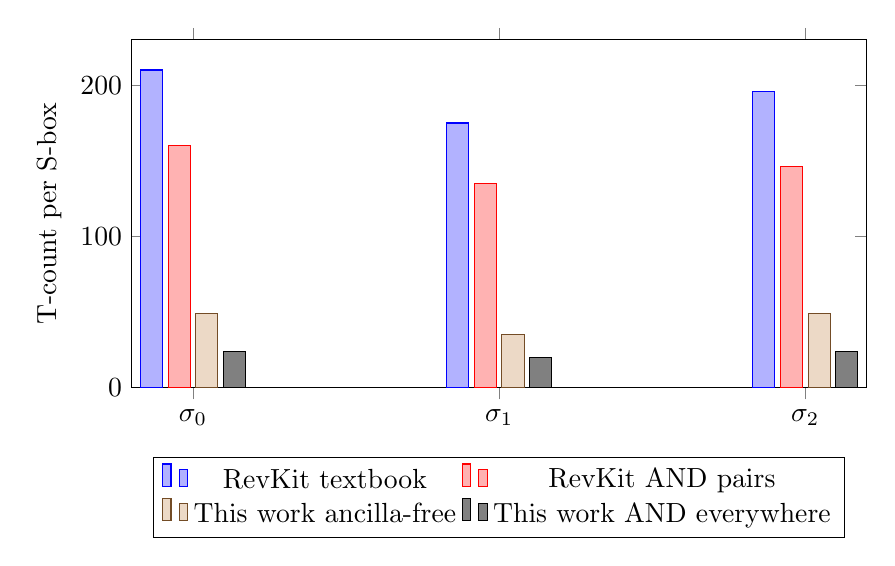
\begin{tikzpicture}
\begin{axis}[
  ybar, bar width=8pt,
  symbolic x coords={$\sigma_0$,$\sigma_1$,$\sigma_2$},
  xtick=data,
  ylabel={T-count per S-box},
  legend style={at={(0.5,-0.2)},anchor=north,legend columns=2},
  width=0.9\textwidth, height=6cm,
  ymin=0, ymax=230
]
\addplot coordinates {($\sigma_0$,210) ($\sigma_1$,175) ($\sigma_2$,196)};
\addplot coordinates {($\sigma_0$,160) ($\sigma_1$,135) ($\sigma_2$,146)};
\addplot coordinates {($\sigma_0$,49) ($\sigma_1$,35) ($\sigma_2$,49)};
\addplot coordinates {($\sigma_0$,24) ($\sigma_1$,20) ($\sigma_2$,24)};
\legend{RevKit textbook, RevKit AND pairs, This work ancilla-free, This work AND everywhere}
\end{axis}
\end{tikzpicture}
\caption{T-count per S-box. The first two bars are the RevKit baseline, the last two this work.}
\label{fig:tcount-per-sbox}
\end{figure}

\section{The Full Encryption Circuit}
\label{sec:full-circuit}

\subsection{Architecture}

The key takes 128 qubits and the state 64, with $\sigma_0$, $\sigma_2$ and the AND-gadget mode adding ancillas on a per-cell basis. Several operations cost nothing at all, because they are permutations of wires: ShuffleCells $\tau$, the tweak permutation $h$, the rotation inside $\omega$, the rotation in $o$, and the output permutation left over by our MixColumns circuit. All of them are handled by relabelling the logical-to-physical qubit map. NOT gates commute through the targets of CNOT and Toffoli gates, so we hold them back until their qubit is next needed as a control; plaintext loading, round constants and tweak constants then merge into a single layer. In the key-search setting the tweak is classical and known, which lets the whole tweak schedule be precomputed and leaves only NOT gates behind. Table~\ref{tab:round-by-round} reports the variant that keeps the tweak in a quantum register.

\subsection{MixColumns}

The matrix itself was not taken on trust. We probe it out of the verified reference implementation on unit inputs, confirm that it is involutory with row weight 3, and only then synthesise a circuit for it. The synthesis reduces the matrix to a permutation matrix rather than to the identity, by randomised greedy row reduction, with the leftover permutation absorbed into the qubit map. Across 40\,000 restarts the best result uses 24 CNOT gates per column at depth 6, so 96 per layer;

\subsection{Resources}

Table~\ref{tab:full-circuit} lists the complete circuit for every S-box and every round number. Taking $\sigma_1$ with $r=7$ as the example: without ancillas the circuit occupies 192 qubits and 8\,960 T gates at T-depth 320, while with AND gadgets it occupies 208 qubits and 5\,120 T gates at T-depth 160, with 1\,280 measurements along the way. The gadget version has 42.9\% fewer T gates and 50.0\% less T-depth; what it pays is 16 extra qubits and a slightly greater full depth, 1\,370 against 1\,226, since every gadget inserts a CNOT and a measurement layer. Set beside the RevKit baseline, the T-count improves by a factor of 8.8. Every Toffoli gate sits in one of the $2r+2=16$ S-box layers, and those layers dominate the CNOT budget as well (Figure~\ref{fig:cnot-breakdown}): 4\,608 of the 7\,268 CNOT gates, or 63.4\%, against 1\,440 for MixColumns and 1\,216 for key addition.

\begin{table}[htbp]
\centering
\caption{Complete QARMA-64 encryption circuit (classical tweak). Depth is the full Clifford+T depth.}
\label{tab:full-circuit}
\scriptsize
\begin{tabular}{llcccccccc}
\toprule
Mode & S-box & $r$ & Qubits & Toffoli & AND & CNOT & NOT & T-count & T-depth (Depth) \\
\midrule
\multirow{9}{*}{textbook 7-T}
& $\sigma_0$ & 5 & 208 & 1\,344 & 0 & 5\,284 & 1\,714 & 9\,408 & 324 (1147) \\
& $\sigma_0$ & 6 & 208 & 1\,568 & 0 & 6\,148 & 1\,998 & 10\,976 & 378 (1339) \\
& $\sigma_0$ & 7 & 208 & 1\,792 & 0 & 7\,012 & 2\,302 & 12\,544 & 432 (1530) \\
& $\sigma_1$ & 5 & 192 & 960 & 0 & 5\,476 & 1\,338 & 6\,720 & 240 (918) \\
& $\sigma_1$ & 6 & 192 & 1\,120 & 0 & 6\,372 & 1\,558 & 7\,840 & 280 (1072) \\
& $\sigma_1$ & 7 & 192 & 1\,280 & 0 & 7\,268 & 1\,798 & 8\,960 & 320 (1226) \\
& $\sigma_2$ & 5 & 208 & 1\,344 & 0 & 5\,476 & 1\,388 & 9\,408 & 324 (1150) \\
& $\sigma_2$ & 6 & 208 & 1\,568 & 0 & 6\,372 & 1\,608 & 10\,976 & 378 (1342) \\
& $\sigma_2$ & 7 & 208 & 1\,792 & 0 & 7\,268 & 1\,848 & 12\,544 & 432 (1534) \\
\midrule
\multirow{9}{*}{AND everywhere}
& $\sigma_0$ & 5 & 224 & 0 & 1\,152 & 6\,244 & 1\,714 & 4\,608 & 121 (1219) \\
& $\sigma_0$ & 6 & 224 & 0 & 1\,344 & 7\,268 & 1\,998 & 5\,376 & 141 (1423) \\
& $\sigma_0$ & 7 & 224 & 0 & 1\,536 & 8\,292 & 2\,302 & 6\,144 & 161 (1626) \\
& $\sigma_1$ & 5 & 208 & 0 & 960 & 6\,436 & 1\,338 & 3\,840 & 120 (1026) \\
& $\sigma_1$ & 6 & 208 & 0 & 1\,120 & 7\,492 & 1\,558 & 4\,480 & 140 (1198) \\
& $\sigma_1$ & 7 & 208 & 0 & 1\,280 & 8\,548 & 1\,798 & 5\,120 & 160 (1370) \\
& $\sigma_2$ & 5 & 224 & 0 & 1\,152 & 6\,436 & 1\,388 & 4\,608 & 121 (1222) \\
& $\sigma_2$ & 6 & 224 & 0 & 1\,344 & 7\,492 & 1\,608 & 5\,376 & 141 (1426) \\
& $\sigma_2$ & 7 & 224 & 0 & 1\,536 & 8\,548 & 1\,848 & 6\,144 & 161 (1630) \\
\midrule
RevKit, textbook 7-T & $\sigma_1$ & 7 & 208 & 6\,400 & 0 & 5\,220 & 1\,044 & 44\,800 & 1584 (4413) \\
RevKit, AND pairs & $\sigma_1$ & 7 & 208 & 4\,352 & 1\,024 & 5\,220 & 1\,044 & 34\,560 & 1216 (3965) \\
RevKit, AND everywhere & $\sigma_1$ & 7 & 224 & 0 & 5\,376 & 9\,572 & 1\,044 & 21\,504 & 608 (4782) \\
\bottomrule
\end{tabular}
\end{table}

\begin{table}[htbp]
\centering
\caption{Round-by-round resources with AND gadgets ($\sigma_1$, $r=7$, 208 qubits). Depths are per segment; the last row is the whole circuit.}
\label{tab:round-by-round}
\scriptsize
\begin{tabular}{lcccccccc}
\toprule
Segment & NOT & CNOT & AND & T-count & Clifford+T total & T-depth & Depth \\
\midrule
Load $P$, whitening $\oplus w^0$ & 34 & 64 & 0 & 0 & 98 & 0 & 2 \\
$R_0$ (short) & 77 & 432 & 80 & 320 & 1\,789 & 10 & 81 \\
$R_1$ & 112 & 528 & 80 & 320 & 1\,920 & 10 & 87 \\
$R_2$ & 114 & 528 & 80 & 320 & 1\,922 & 10 & 87 \\
$R_3$ & 111 & 528 & 80 & 320 & 1\,919 & 10 & 87 \\
$R_4$ & 109 & 528 & 80 & 320 & 1\,917 & 10 & 87 \\
$R_5$ & 108 & 528 & 80 & 320 & 1\,916 & 10 & 87 \\
$R_6$ & 122 & 528 & 80 & 320 & 1\,930 & 10 & 87 \\
Central $R$ & 115 & 529 & 80 & 320 & 1\,924 & 10 & 87 \\
Pseudo-reflector ($\tau$, $Q$, $\oplus k^1$, $\tau^{-1}$) & 0 & 160 & 0 & 0 & 160 & 0 & 7 \\
Central $R$ & 115 & 529 & 80 & 320 & 1\,924 & 10 & 86 \\
$R_6$ & 114 & 528 & 80 & 320 & 1\,922 & 10 & 86 \\
$R_5$ & 112 & 528 & 80 & 320 & 1\,920 & 10 & 86 \\
$R_4$ & 109 & 528 & 80 & 320 & 1\,917 & 10 & 86 \\
$R_3$ & 119 & 528 & 80 & 320 & 1\,927 & 10 & 86 \\
$R_2$ & 114 & 528 & 80 & 320 & 1\,922 & 10 & 86 \\
$R_1$ & 108 & 528 & 80 & 320 & 1\,916 & 10 & 86 \\
$R_0$ (short) & 105 & 432 & 80 & 320 & 1\,817 & 10 & 80 \\
Whitening $\oplus w^1$, key restore & 0 & 66 & 0 & 0 & 66 & 0 & 3 \\
\midrule
\textbf{Whole circuit} & \textbf{1\,798} & \textbf{8\,548} & \textbf{1\,280} & \textbf{5\,120} & \textbf{30\,826} & \textbf{160} & \textbf{1370} \\
\bottomrule
\end{tabular}
\end{table}

\begin{figure}[htbp]
\centering
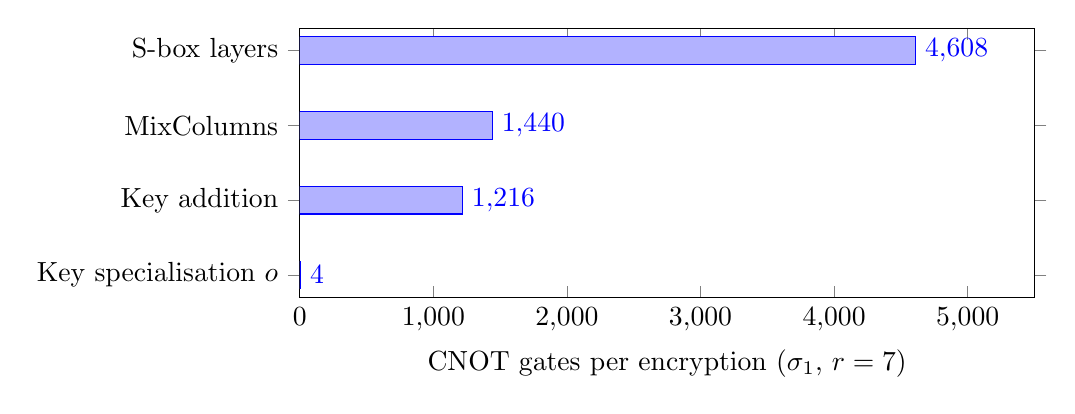
\begin{tikzpicture}
\begin{axis}[
  xbar, bar width=10pt,
  symbolic y coords={Key specialisation $o$,Key addition,MixColumns,S-box layers},
  ytick=data,
  xlabel={CNOT gates per encryption ($\sigma_1$, $r=7$)},
  width=0.9\textwidth, height=5cm,
  nodes near coords, nodes near coords align={horizontal},
  xmin=0, xmax=5500
]
\addplot coordinates {(4,Key specialisation $o$) (1216,Key addition) (1440,MixColumns) (4608,S-box layers)};
\end{axis}
\end{tikzpicture}
\caption{Where the CNOT gates go in one encryption ($\sigma_1$, $r=7$).}
\label{fig:cnot-breakdown}
\end{figure}

\begin{table}[htbp]
\centering
\caption{Variant with a quantum tweak register (AND gadgets), where the tweak schedule runs in the circuit and the tweak register is restored.}
\label{tab:quantum-tweak}
\small
\begin{tabular}{lcccccc}
\toprule
S-box & $r$ & Qubits & CNOT & NOT & T-count & T-depth (Depth) \\
\midrule
\multirow{3}{*}{$\sigma_0$} & 5 & 288 & 7\,082 & 1\,600 & 4\,608 & 121 (1228) \\
 & 6 & 288 & 8\,248 & 1\,896 & 5\,376 & 141 (1433) \\
 & 7 & 288 & 9\,414 & 2\,188 & 6\,144 & 161 (1639) \\
\multirow{3}{*}{$\sigma_1$} & 5 & 272 & 7\,274 & 1\,224 & 3\,840 & 120 (1036) \\
 & 6 & 272 & 8\,472 & 1\,456 & 4\,480 & 140 (1209) \\
 & 7 & 272 & 9\,670 & 1\,684 & 5\,120 & 160 (1384) \\
\multirow{3}{*}{$\sigma_2$} & 5 & 288 & 7\,274 & 1\,244 & 4\,608 & 121 (1232) \\
 & 6 & 288 & 8\,472 & 1\,476 & 5\,376 & 141 (1438) \\
 & 7 & 288 & 9\,670 & 1\,704 & 6\,144 & 161 (1643) \\
\bottomrule
\end{tabular}
\end{table}

\section{Grover Key Search}
\label{sec:grover}

\subsection{Oracle, comparator and diffusion}

A 128-bit key against a 64-bit block means that $s$ plaintext--ciphertext pairs leave $2^{128-64s}$ false keys in expectation: one for $s=2$, and $2^{-64}$ for $s=3$. The oracle of Figure~\ref{fig:grover-oracle} runs $s$ encryptions sharing a single key register, flips each state qubit whose expected ciphertext bit is 0, and computes the AND of all $64s$ qubits onto a phase qubit prepared in $|-\rangle$. That AND is a logarithmic-depth tree of $64s-1$ AND gadgets at 4 T each, and its uncomputation is free; the encryptions are then run backwards. Diffusion is the usual $H^{\otimes 128}X^{\otimes 128}$, a 127-controlled $Z$ drawn from the same ancilla pool, and the inverses of both.

\subsection{Verification}

\begin{figure}[htbp]
\centering
\begin{quantikz}
\lstick{$|0\rangle^{\otimes 128}$ key} & \gate{H^{\otimes 128}} & \gate[3]{U_{\mathrm{Enc}}^{\otimes s}} & \qw & \qw & \gate[3]{U_{\mathrm{Enc}}^{\dagger\,\otimes s}} & \gate{D} & \qw \\
\lstick{$|0\rangle^{\otimes 64s}$ states} & \qw & & \gate{X_C} & & & \qw & \qw \\
\lstick{$|0\rangle^{\otimes(64s-1)}$ AND tree} & \qw & & \gate[2]{\text{AND tree}} & & & \qw & \qw \\
\lstick{$|0\rangle$ phase} & \gate{H} & \qw & & \qw & \qw & \qw & \meter{}
\end{quantikz}
\caption{Grover key search on QARMA-64 with $s$ plaintext--ciphertext pairs, repeated $\left\lfloor \frac{\pi}{4}2^{64}\right\rfloor \approx 2^{63.65}$ times.}
\label{fig:grover-oracle}
\end{figure}

\subsection{Cost}

Table~\ref{tab:grover-cost} gives per-iteration and total costs over $\left\lfloor \frac{\pi}{4}2^{64}\right\rfloor = 14\,488\,038\,916\,154\,245\,684 \approx 2^{63.65}$ iterations. With three pairs, AND gadgets cut the per-iteration T-count from 58\,198 to 31\,988 (45.0\%) and the T-depth from 758 to 334 (55.9\%), for 560 qubits instead of 512. The full attack then costs $2^{81.19}$ Clifford+T gates, $2^{78.62}$ of them T gates, at depth $2^{75.19}$ and DW-cost $2^{84.32}$.

It pays to be precise about what the gadgets actually buy here. They roughly halve T-count and T-depth, yet the total gate count barely moves, $2^{81.11}$ without them against $2^{81.19}$ with them. The reason is that Clifford gates dominate that total, and each gadget swaps T gates for Clifford gates, a measurement and one more CNOT. Under a surface-code cost model, where distillation is the bottleneck, T-count and T-depth are what matter and the gadgets are better . 

\begin{table}[htbp]
\centering
\caption{Grover key search ($\sigma_1$, $r=7$). Per-iteration columns describe one oracle plus diffusion; attack columns are $\log_2$ totals over all iterations.}
\label{tab:grover-cost}
\small
\begin{tabular}{llccccc|ccc}
\toprule
& & \multicolumn{5}{c|}{Per iteration} & \multicolumn{3}{c}{Full attack ($\log_2$)} \\
Mode & $s$ & Qubits & Toffoli & AND & T-count & T-depth (Depth) & G-cost & T-count & Depth \\
\midrule
\multirow{3}{*}{textbook 7-T}
 & 1 & 320 & 2\,938 & 0 & 20\,566 & 743 (2716) & 79.59 & 77.98 & 75.06 \\
 & 2 & 384 & 5\,626 & 0 & 39\,382 & 751 (2738) & 80.54 & 78.92 & 75.07 \\
 & 3 & 512 & 8\,314 & 0 & 58\,198 & 758 (2756) & 81.11 & 79.48 & 75.08 \\
\midrule
\multirow{3}{*}{AND everywhere}
 & 1 & 336 & 0 & 2\,749 & 10\,996 & 332 (2947) & 79.65 & 77.08 & 75.18 \\
 & 2 & 416 & 0 & 5\,373 & 21\,492 & 333 (2960) & 80.62 & 78.04 & 75.18 \\
 & 3 & 560 & 0 & 7\,997 & 31\,988 & 334 (2972) & 81.19 & 78.62 & 75.19 \\
\bottomrule
\end{tabular}
\end{table}

\subsection{Depth-limited attacks}

Should the total depth $I \cdot d$ exceed $MAXDEPTH$, the key space has to be divided over $S = (Id/m_d)^2$ parallel instances, and the total gate count becomes $G_{m_d} = I^2 g d / m_d$. Table~\ref{tab:depth-limited} and Figure~\ref{fig:depth-limited} work this through. At $m_d = 2^{40}$ and $2^{64}$ the attack costs $2^{116.38}$ and $2^{92.38}$ gates, in both cases below NIST's AES-128 reference of $2^{170}/m_d$. At $2^{96}$ the limit stops binding altogether, no parallelisation is needed, and the reference formula ceases to mean much in that regime. One consequence deserves attention. As soon as the depth limit does bind, the ordering of our two variants flips: parallelisation cost scales with the square of the depth, so the marginally deeper AND-gadget circuit ends up marginally more expensive than the ancilla-free one (Table~\ref{tab:depth-limited}). That is a real trade-off rather than a rounding artefact, and it is why both variants are carried through every table. A caveat on interpretation: these are gate counts for a 128-bit key search and nothing more. They say nothing directly about QARMA-64's security margin, which depends on data complexity and on the designers' own claims~\cite{avanzi2017qarma}.

\begin{table}[htbp]
\centering
\caption{Depth-limited Grover key search ($\sigma_1$, $r=7$, 3 pairs). $S$ = parallel instances, $W_{\mathrm{tot}} = S\cdot W$.}
\label{tab:depth-limited}
\small
\begin{tabular}{llcccc}
\toprule
$MAXDEPTH$ & Mode & $S$ ($\log_2$) & $W_{\mathrm{tot}}$ ($\log_2$) & $G$ ($\log_2$) & AES-128 reference $2^{170}/m_d$ \\
\midrule
\multirow{2}{*}{$2^{40}$} & textbook 7-T & 70.16 & 79.16 & 116.19 & $2^{130}$ \\
 & AND everywhere & 70.38 & 79.51 & 116.38 & $2^{130}$ \\
\multirow{2}{*}{$2^{64}$} & textbook 7-T & 22.16 & 31.16 & 92.19 & $2^{106}$ \\
 & AND everywhere & 22.38 & 31.51 & 92.38 & $2^{106}$ \\
\multirow{2}{*}{$2^{96}$} & textbook 7-T & 0.00 & 9.00 & 81.11 & $2^{74}$ \\
 & AND everywhere & 0.00 & 9.13 & 81.19 & $2^{74}$ \\
\bottomrule
\end{tabular}
\end{table}

\begin{figure}[htbp]
\centering
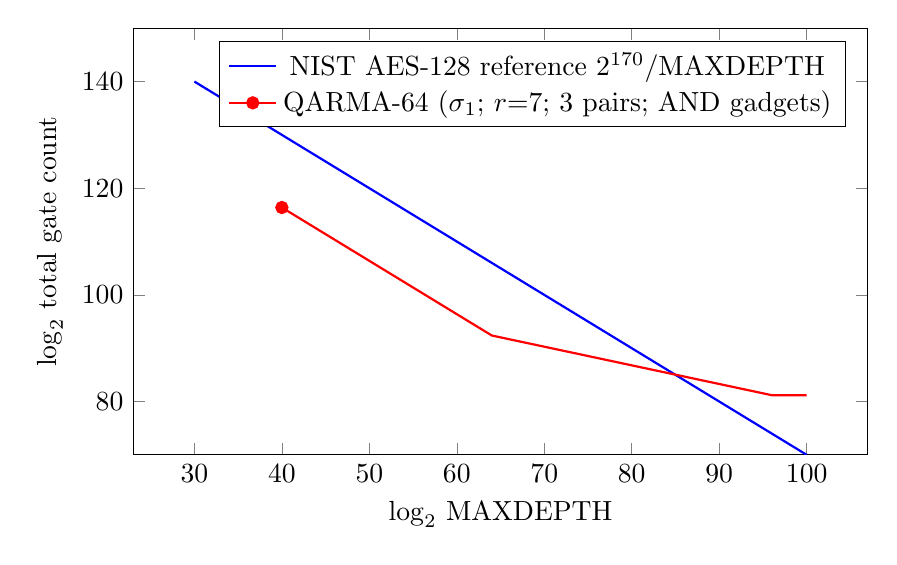
\begin{tikzpicture}
\begin{axis}[
  xlabel={$\log_2$ MAXDEPTH}, ylabel={$\log_2$ total gate count},
  width=0.9\textwidth, height=7cm,
  domain=30:100, samples=200,
  legend pos=north east,
  ymin=70, ymax=150
]
\addplot[thick, blue] {170-x};
\addlegendentry{NIST AES-128 reference $2^{170}/\mathrm{MAXDEPTH}$}
\addplot[thick, red, mark=*, mark repeat=40] coordinates {(40,116.38) (64,92.38) (96,81.19) (100,81.19)};
\addlegendentry{QARMA-64 ($\sigma_1$; $r{=}7$; 3 pairs; AND gadgets)}
\end{axis}
\end{tikzpicture}
\caption{Total gate count against the depth limit.}
\label{fig:depth-limited}
\end{figure}



\begin{enumerate}
\item \textbf{Reference cipher.} Structural self-tests ($\sigma_0$, $\sigma_1$ involutory, $M^2=I$, tweak update invertible) and all nine published test vectors.
\item \textbf{Gadgets as unitaries.} The 7-T Toffoli equals $CCX$ exactly; the AND compute is exact on all four $|a,b,0\rangle$ inputs with amplitude $+1$; the uncompute restores the input state in both branches, each with probability exactly $1/2$; Equation~\eqref{eq:borrowed-toffoli} is exact on random superpositions.
\item \textbf{S-box search.} Unit tests establish that coset canonicalisation is invariant under left affine multiplication and separates distinct cosets, and known-answer tests recover planted products of $k=1,\ldots,4$ generalised Toffoli gates with exactly $k$.
\item \textbf{S-box circuits.} Each is checked on all 16 inputs with ancillas required to return to $|0\rangle$, and additionally in every measurement branch (up to 64 sampled branches for the largest) against the ideal permutation on a random superposition; the largest deviation observed anywhere was $\sim 10^{-16}$.
\item \textbf{MixColumns.} The matrix is probed from the reference, checked involutory, and the circuit is checked on 500 random columns.
\item \textbf{Full cipher.} 39 configurations (S-box $\times$ rounds $\times$ gadget mode $\times$ classical/quantum tweak $\times$ baseline) each reproduce the published ciphertext, with key, tweak and ancillas restored.
\item \textbf{Grover.} Oracle marking and uncomputation as described in Section~\ref{sec:grover}, plus the toy Grover run.
\end{enumerate}

\begin{table}[htbp]
\centering
\caption{End-to-end verification against the published QARMA-64 test vectors, for the ancilla-free and the AND-gadget circuits.}
\label{tab:test-vectors}
\small
\begin{tabular}{llccc}
\toprule
S-box & $r$ & Published ciphertext & Ancilla-free circuit & AND-gadget circuit \\
\midrule
$\sigma_0$ & 5 & \texttt{3ee99a6c82af0c38} & \texttt{3ee99a6c82af0c38} & \texttt{3ee99a6c82af0c38} \checkmark \\
$\sigma_0$ & 6 & \texttt{9f5c41ec525603c9} & \texttt{9f5c41ec525603c9} & \texttt{9f5c41ec525603c9} \checkmark \\
$\sigma_0$ & 7 & \texttt{bcaf6c89de930765} & \texttt{bcaf6c89de930765} & \texttt{bcaf6c89de930765} \checkmark \\
$\sigma_1$ & 5 & \texttt{544b0ab95bda7c3a} & \texttt{544b0ab95bda7c3a} & \texttt{544b0ab95bda7c3a} \checkmark \\
$\sigma_1$ & 6 & \texttt{a512dd1e4e3ec582} & \texttt{a512dd1e4e3ec582} & \texttt{a512dd1e4e3ec582} \checkmark \\
$\sigma_1$ & 7 & \texttt{edf67ff370a483f2} & \texttt{edf67ff370a483f2} & \texttt{edf67ff370a483f2} \checkmark \\
$\sigma_2$ & 5 & \texttt{c003b93999b33765} & \texttt{c003b93999b33765} & \texttt{c003b93999b33765} \checkmark \\
$\sigma_2$ & 6 & \texttt{270a787275c48d10} & \texttt{270a787275c48d10} & \texttt{270a787275c48d10} \checkmark \\
$\sigma_2$ & 7 & \texttt{5c06a7501b63b2fd} & \texttt{5c06a7501b63b2fd} & \texttt{5c06a7501b63b2fd} \checkmark \\
\bottomrule
\end{tabular}
\end{table}

\section{Discussion}

\subsection{Limitations}

Everything reported here is at the logical level. Error correction, routing and magic-state distillation overheads are excluded, as they usually are in this literature~\cite{grassl2016applying,jaques2020implementing}, and the zero-T uncomputation assumes mid-circuit measurement with classical feed-forward. The AND-gadget circuits buy T gates with qubits, 16 or 32 extra per state register, which is a good trade under most fault-tolerant cost models and a poor one if width is taken as main  constraint. Our minimality result covers ancilla-free circuits only, and we prove no lower bound on T-count whatsoever; the multiplicative complexity of the S-boxes is the natural tool for that and we did not pursue it. Grover search, lastly, is the generic attack in the Q1 model. In the Q2 model, where the adversary queries the keyed primitive in superposition, Even--Mansour-like constructions fall to far stronger attacks based on Simon's algorithm~\cite{kuwakado2012security,kaplan2016breaking}, and no cost model of this kind speaks to that. QARMAv2~\cite{avanzi2023qarmav2} revises the design and deserves its own analysis; the tooling here would carry over with little change.

\section{Conclusion}

What began as an attempt to avoid paying 21 T gates for a single $C^3X$ and covering the  whole cipher: exact Toffoli counts for the S-boxes, a careful application of Gidney's temporary-AND construction, and a Grover oracle that was built and tested. Together these bring one encryption down to 5\,120 T gates at T-depth 160, a factor of 8.8 below a RevKit baseline, and place Grover key recovery at $2^{81.19}$ Clifford+T gates on 560 logical qubits.

\appendix


\section{Gate Sequences}\label{app:gate-sequences}

Sequences are applied in the order $1,2,3,\ldots$ (read column by column); $CX(a\to b)$ has control $a$ and target $b$, and $a$ denotes the ancilla wire.



\begin{table}[htbp]
\centering
\caption{$\sigma_1$ (5 Toffoli, ancilla-free).}
\label{tab:sigma1-full-gates}
\small
\begin{tabular}{cl cl cl}
\toprule
\# & Gate & \# & Gate & \# & Gate \\
\midrule
1 & $X(x_2)$ & 11 & $CX(x_3\to x_0)$ & 21 & $CX(x_2\to x_0)$ \\
2 & $X(x_3)$ & 12 & $CX(x_2\to x_3)$ & 22 & $CX(x_3\to x_1)$ \\
3 & $CX(x_2\to x_0)$ & 13 & $X(x_3)$ & 23 & $X(x_2)$ \\
4 & $CX(x_3\to x_1)$ & 14 & $CCX(x_0,x_1\to x_2)$ & 24 & $CCX(x_0,x_1\to x_2)$ \\
5 & $CCX(x_0,x_1\to x_2)$ & 15 & $CX(x_3\to x_0)$ & 25 & $CX(x_2\to x_0)$ \\
6 & $CX(x_2\to x_0)$ & 16 & $CX(x_0\to x_2)$ & 26 & $CX(x_1\to x_2)$ \\
7 & $CX(x_1\to x_2)$ & 17 & $CX(x_2\to x_1)$ & 27 & $CX(x_3\to x_1)$ \\
8 & $CX(x_3\to x_1)$ & 18 & $CCX(x_0,x_1\to x_2)$ & 28 & $X(x_3)$ \\
9 & $CCX(x_0,x_1\to x_2)$ & 19 & $CX(x_1\to x_0)$ & & \\
10 & $CX(x_2\to x_1)$ & 20 & $CX(x_1\to x_3)$ & & \\
\bottomrule
\end{tabular}
\end{table}

\begin{table}[htbp]
\centering
\caption{$\sigma_0$ (4 Toffoli + one $C^3X$).}
\label{tab:sigma0-full-gates}
\small
\begin{tabular}{cl cl cl}
\toprule
\# & Gate & \# & Gate & \# & Gate \\
\midrule
1 & $CX(x_2\to x_0)$ & 11 & $CX(x_3\to x_1)$ & 21 & $X(x_2)$ \\
2 & $CX(x_2\to x_1)$ & 12 & $CX(x_2\to x_3)$ & 22 & $CCX(x_0,x_1\to x_2)$ \\
3 & $X(x_1)$ & 13 & $CCX(x_0,x_1\to x_2)$ & 23 & $CX(x_0\to x_2)$ \\
4 & $C^3X(x_0,x_1,x_2\to x_3)$ & 14 & $X(x_1)$ & 24 & $CX(x_2\to x_3)$ \\
5 & $CX(x_3\to x_2)$ & 15 & $X(x_3)$ & 25 & $CX(x_3\to x_1)$ \\
6 & $CX(x_1\to x_3)$ & 16 & $CX(x_2\to x_0)$ & 26 & $CX(x_1\to x_0)$ \\
7 & $CX(x_2\to x_0)$ & 17 & $CX(x_0\to x_1)$ & 27 & $CX(x_3\to x_2)$ \\
8 & $CX(x_2\to x_1)$ & 18 & $CX(x_3\to x_0)$ & 28 & $X(x_1)$ \\
9 & $X(x_0)$ & 19 & $CCX(x_0,x_1\to x_2)$ & 29 & $X(x_2)$ \\
10 & $CCX(x_0,x_1\to x_2)$ & 20 & $CX(x_2\to x_0)$ & & \\
\bottomrule
\end{tabular}
\end{table}

\begin{table}[htbp]
\centering
\caption{$\sigma_2$ (4 Toffoli + one $C^3X$); $\sigma_2^{-1}$ reverses the order.}
\label{tab:sigma2-full-gates}
\small
\begin{tabular}{cl cl cl}
\toprule
\# & Gate & \# & Gate & \# & Gate \\
\midrule
1 & $CX(x_0\to x_3)$ & 11 & $CCX(x_0,x_1\to x_2)$ & 21 & $CCX(x_0,x_1\to x_2)$ \\
2 & $CX(x_1\to x_0)$ & 12 & $CX(x_2\to x_1)$ & 22 & $X(x_0)$ \\
3 & $CX(x_2\to x_0)$ & 13 & $CX(x_3\to x_2)$ & 23 & $X(x_1)$ \\
4 & $C^3X(x_0,x_1,x_2\to x_3)$ & 14 & $CX(x_2\to x_0)$ & 24 & $CX(x_3\to x_0)$ \\
5 & $CX(x_3\to x_1)$ & 15 & $CCX(x_0,x_1\to x_2)$ & 25 & $CX(x_0\to x_2)$ \\
6 & $CCX(x_0,x_1\to x_2)$ & 16 & $X(x_0)$ & 26 & $CX(x_2\to x_3)$ \\
7 & $X(x_3)$ & 17 & $X(x_3)$ & 27 & $CX(x_3\to x_1)$ \\
8 & $CX(x_3\to x_1)$ & 18 & $CX(x_2\to x_0)$ & 28 & $CX(x_1\to x_2)$ \\
9 & $CX(x_0\to x_3)$ & 19 & $CX(x_2\to x_3)$ & & \\
10 & $CX(x_2\to x_0)$ & 20 & $CX(x_3\to x_1)$ & & \\
\bottomrule
\end{tabular}
\end{table}

\begin{table}[htbp]
\centering
\caption{MixColumns gate sequence on wires $v_0,\ldots,v_{15}$.}
\label{tab:mixcolumns-gates}
\small
\begin{tabular}{cl cl cl cl}
\toprule
\# & Gate & \# & Gate & \# & Gate & \# & Gate \\
\midrule
1 & $CX(v_{10}\to v_2)$ & 7 & $CX(v_9\to v_{12})$ & 13 & $CX(v_4\to v_{11})$ & 19 & $CX(v_2\to v_5)$ \\
2 & $CX(v_{15}\to v_{10})$ & 8 & $CX(v_0\to v_8)$ & 14 & $CX(v_4\to v_3)$ & 20 & $CX(v_2\to v_{13})$ \\
3 & $CX(v_{12}\to v_4)$ & 9 & $CX(v_1\to v_{12})$ & 15 & $CX(v_{12}\to v_4)$ & 21 & $CX(v_{10}\to v_2)$ \\
4 & $CX(v_7\to v_{10})$ & 10 & $CX(v_{13}\to v_0)$ & 16 & $CX(v_8\to v_7)$ & 22 & $CX(v_{14}\to v_1)$ \\
5 & $CX(v_6\to v_{14})$ & 11 & $CX(v_{11}\to v_6)$ & 17 & $CX(v_8\to v_{15})$ & 23 & $CX(v_{14}\to v_9)$ \\
6 & $CX(v_3\to v_6)$ & 12 & $CX(v_5\to v_0)$ & 18 & $CX(v_0\to v_8)$ & 24 & $CX(v_6\to v_{14})$ \\
\bottomrule
\end{tabular}
\end{table}

\begin{figure}[htbp]
\centering
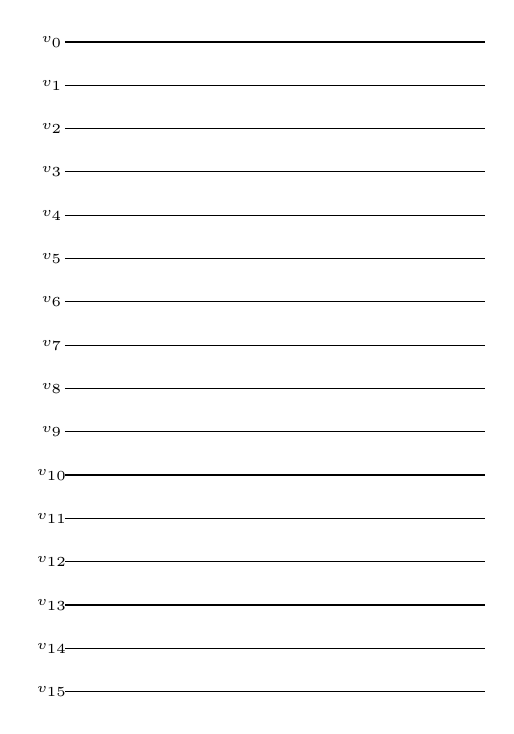
\begin{tikzpicture}[scale=0.55, every node/.style={font=\tiny}]
  \foreach \i in {0,...,15} {
    \node at (0,-\i) {$v_{\i}$};
    \draw (0.3,-\i) -- (10,-\i);
  }
\end{tikzpicture}
\caption{One MixColumns column: 24 CNOT gates, depth 6. Wires carry the input bits (a relabelling); wire $v_w$ ends holding $y_{\lfloor w/4\rfloor,\, w\bmod 4}$. The full gate sequence is given in Table~\ref{tab:mixcolumns-gates}.}
\label{fig:mixcolumns}
\end{figure}

% Flush all gate-sequence floats before beginning the notation appendix.
% Without this, LaTeX may place the notation subsection between the tables.
\clearpage
\subsection{Notation}

The following notation is used throughout the paper:

\begin{itemize}
    \item $K$: 128-bit secret key.
    \item $P$: 64-bit plaintext.
    \item $C$: 64-bit ciphertext.
    \item $T$: 64-bit tweak.
    \item $r$: Number of forward rounds in QARMA-64.
    \item $\sigma_0,\sigma_1,\sigma_2$: QARMA-64 S-boxes.
    \item $X$: NOT gate.
    \item $CX$: Controlled-NOT gate.
    \item $CCX$: Toffoli gate.
    \item $C^3X$: Three-controlled NOT gate.
    \item $k$: Key size in bits.
    \item $s$: Number of plaintext--ciphertext pairs used in the Grover search.
    \item $O_f$: Grover oracle that marks the key satisfying the required plaintext--ciphertext conditions.
    \item $D$: Grover diffusion operator that amplifies the marked state.
    \item $DO_f$: One complete Grover iteration, consisting of the oracle $O_f$ followed by the diffusion operator $D$.
    \item T-count: Total number of $T$ gates in a circuit.
    \item T-depth: Number of sequential layers containing $T$ gates.
    \item $G$-cost: Total gate count of the circuit.
    \item DW-cost: Circuit depth multiplied by circuit width.
\end{itemize}









\begin{thebibliography}{99}

\bibitem{avanzi2017qarma} R. Avanzi. The QARMA block cipher family. Almost MDS matrices over rings with zero divisors, nearly symmetric Even--Mansour constructions with non-involutory central rounds, and search heuristics for low-latency S-boxes. \emph{IACR Transactions on Symmetric Cryptology}, 2017(1):4--44, 2017.

\bibitem{avanzi2023qarmav2} R. Avanzi, S. Banik, O. Dunkelman, M. Eichlseder, S. Ghosh, M. Nageler, F. Regazzoni. The QARMAv2 family of tweakable block ciphers. \emph{IACR Transactions on Symmetric Cryptology}, 2023(3):25--73, 2023.

\bibitem{qualcomm2017pac} Qualcomm Technologies, Inc. Pointer Authentication on ARMv8.3: Design and Analysis of the New Software Security Instructions. White paper, January 2017.

\bibitem{grover1996fast} L. K. Grover. A fast quantum mechanical algorithm for database search. In \emph{Proc. 28th ACM STOC}, pages 212--219, 1996.

\bibitem{boyer1998tight} M. Boyer, G. Brassard, P. H{\o}yer, A. Tapp. Tight bounds on quantum searching. \emph{Fortschritte der Physik}, 46(4--5):493--505, 1998.

\bibitem{zalka1999grovers} C. Zalka. Grover's quantum searching algorithm is optimal. \emph{Physical Review A}, 60(4):2746--2751, 1999.

\bibitem{grassl2016applying} M. Grassl, B. Langenberg, M. Roetteler, R. Steinwandt. Applying Grover's algorithm to AES: quantum resource estimates. In \emph{PQCrypto 2016}, LNCS 9606, pages 29--43. Springer, 2016.

\bibitem{jaques2020implementing} S. Jaques, M. Naehrig, M. Roetteler, F. Virdia. Implementing Grover oracles for quantum key search on AES and LowMC. In \emph{EUROCRYPT 2020}, LNCS 12106, pages 280--310. Springer, 2020.

\bibitem{nist2016submission} National Institute of Standards and Technology. Submission Requirements and Evaluation Criteria for the Post-Quantum Cryptography Standardization Process, December 2016.

\bibitem{gidney2018halving} C. Gidney. Halving the cost of quantum addition. \emph{Quantum}, 2:74, 2018. arXiv:1709.06648.

\bibitem{jones2013lowoverhead} N. C. Jones. Low-overhead constructions for the fault-tolerant Toffoli gate. \emph{Physical Review A}, 87(2):022328, 2013. arXiv:1212.5069.

\bibitem{harrigan2024expressing} M. P. Harrigan, T. Khattar, C. Yuan, A. Peduri, N. Yosri, F. D. Malone, R. Babbush, N. C. Rubin. Expressing and analyzing quantum algorithms with Qualtran. arXiv:2409.04643, 2024. Software: \url{https://github.com/quantumlib/Qualtran}.

\bibitem{nielsen2010quantum} M. A. Nielsen, I. L. Chuang. \emph{Quantum Computation and Quantum Information}. Cambridge University Press, 10th anniversary edition, 2010.

\bibitem{barenco1995elementary} A. Barenco, C. H. Bennett, R. Cleve, D. P. DiVincenzo, N. Margolus, P. Shor, T. Sleator, J. A. Smolin, H. Weinfurter. Elementary gates for quantum computation. \emph{Physical Review A}, 52(5):3457--3467, 1995.

\bibitem{amy2013meetinthemiddle} M. Amy, D. Maslov, M. Mosca, M. Roetteler. A meet-in-the-middle algorithm for fast synthesis of depth-optimal quantum circuits. \emph{IEEE Transactions on Computer-Aided Design of Integrated Circuits and Systems}, 32(6):818--830, 2013.

\bibitem{selinger2013quantum} P. Selinger. Quantum circuits of T-depth one. \emph{Physical Review A}, 87(4):042302, 2013.

\bibitem{dasu2019lighterr} V. A. Dasu, A. Baksi, S. Sarkar, A. Chattopadhyay. LIGHTER-R: optimized reversible circuit implementation for SBoxes. In \emph{32nd IEEE International System-on-Chip Conference (SOCC 2019)}, pages 260--265. IEEE, 2019.

\bibitem{soeken2012revkit} M. Soeken, S. Frehse, R. Wille, R. Drechsler. RevKit: an open source toolkit for the design of reversible circuits. In \emph{Reversible Computation (RC 2011)}, LNCS 7165, pages 64--76. Springer, 2012.

\bibitem{banik2015midori} S. Banik, A. Bogdanov, T. Isobe, K. Shibutani, H. Hiwatari, T. Akishita, F. Regazzoni. Midori: a block cipher for low energy. In \emph{ASIACRYPT 2015}, LNCS 9453, pages 411--436. Springer, 2015.

\bibitem{kuwakado2012security} H. Kuwakado, M. Morii. Security on the quantum-type Even--Mansour cipher. In \emph{Proc. ISITA 2012}, pages 312--316. IEEE, 2012.

\bibitem{kaplan2016breaking} M. Kaplan, G. Leurent, A. Leverrier, M. Naya-Plasencia. Breaking symmetric cryptosystems using quantum period finding. In \emph{CRYPTO 2016}, LNCS 9815, pages 207--237. Springer, 2016.

\end{thebibliography}

\end{document}
